\chapter{Overview of Synthetic Data Generation}
\section{Overview}
In more broad and accepted terms, synthetic data is "any production data applicable to a given situation that are not obtained by direct measurement" according to the McGraw-Hill Dictionary of Scientific and Technical Terms.\\ Synthetic data is not only popular and useful in computer science but it is also important in other business functions/types such as: Healthcare Systems, Fraud Detection Systems etc. In this project, the data synthesis of various real-life data stored into databases is important. In this type of data synthesis, that data is initially analyzed and then transformed, or rather just used in order to generate another set of data, so it isn't really a transformation but rather just a mere "sample" or "pattern" for the synthesized data. \\
Various methods and techniques are used in order to synthesize data. The procedure of this examination, analysis and generation of the real data into synthetic data is explained thoroughly and in more detailed and technical terms in the \nameref{ch:implementation} chapter.\\
Synthetic data does NOT refer to anonymized data, it is often a misconception or a myth, there are various types of data transformations that can happen from real data such as: Anonymized data, artificial data, synthesized data etc. Moreover, there are also subtypes of the types mentioned above, which are of course, more detailed and technical. The image below by \citeauthor{Synthesized_2018}, depicts this in a pretty neat way.
\begin{figure}[H]
	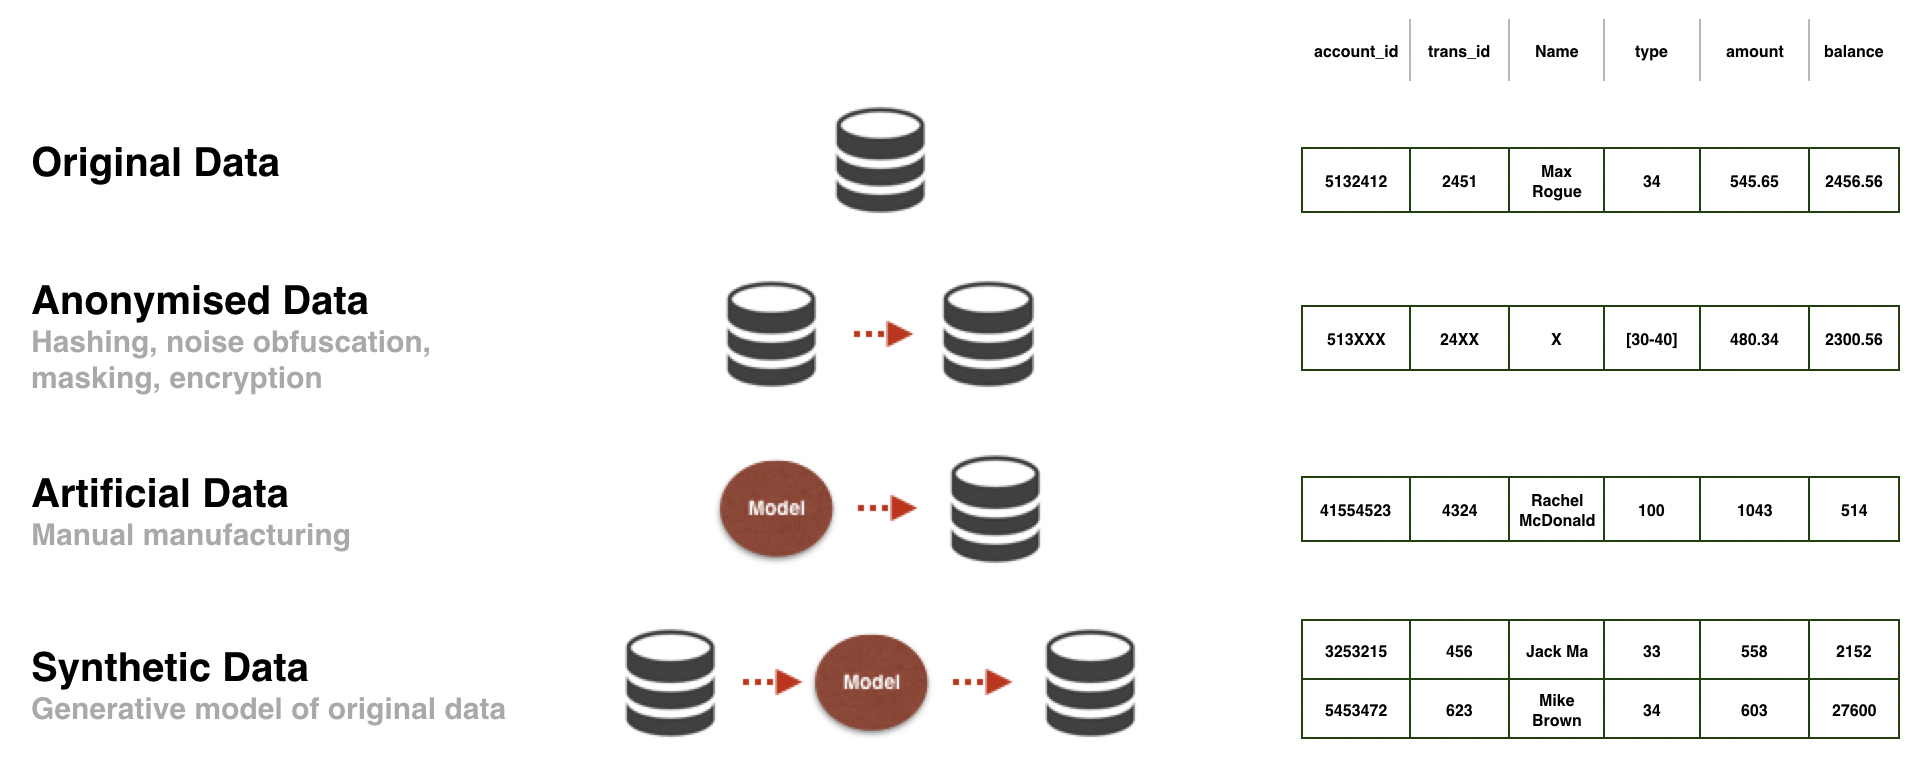
\includegraphics[width=\linewidth]{./Figures/Synthetic_Data/types_of_data_comparison.png}
	\caption{Three approaches to synthetic data, from \citeauthor{Synthesized_2018}}
\end{figure}
\section{Data Synthesization}
\lipsum[6-8]
\noindent\includegraphics[width=3cm]{example-image-a}\qquad
\includegraphics[width=3cm]{example-image-golden}\qquad
\section{Data Generation}
\lipsum[8-9]
\noindent\includegraphics[scale=0.5]{example-image-b} 
\section{Selected Database Related Open Source Tools }
\lipsum[8-9]
\noindent\includegraphics[scale=0.5]{example-image-c} 
\section{Remarks and Further Resources}
\lipsum[8-9]
\noindent\includegraphics[scale=0.5]{example-image-a} 